%!TEX program = xelatex
% 完整编译方法 1 pdflatex -> bibtex -> pdflatex -> pdflatex
% 完整编译方法 2: xelatex -> bibtex -> xelatex -> xelatex
\documentclass[lang=cn,11pt,a4paper,numbers]{elegantpaper}
% \setCJKmainfont[UprightFont = Songti SC Light, BoldFont=Songti SC Bold, ItalicFont=Kaiti SC, BoldItalicFont = Kaiti SC Bold]{Songti SC Regular}
% \setmainfont{Times New Roman}
% \newfontfamily\menlo{Menlo}
\newfontfamily\arial{Arial}
\newcommand{\w}{\boldsymbol w}
\newcommand{\x}{\boldsymbol x}
\newcommand{\g}{\boldsymbol g}
\newcommand{\p}{\boldsymbol p}
\newcommand{\z}{\boldsymbol z}
\newcommand{\intd}{\textrm{d}}
\newcommand{\e}{\textrm{e}}
% \newcommand{\d}{}
\DeclareMathOperator*{\argmax}{arg\,max}
\DeclareMathOperator*{\argmin}{arg\,min}
\usepackage{algorithm}
\usepackage{algorithmic}
\usepackage{tabularx}
\usepackage{multicol}
\usepackage{graphicx}
\usepackage{caption}
\usepackage{url}
\usepackage{amsmath}
% \usepackage{bm}
%%
% \usepackage[T1]{fontenc}
% \usepackage{libertine}
% \usepackage[libertine]{newtxmath}
%%
% \usepackage[T1]{fontenc}
% \usepackage{Alegreya}
%%
% \usepackage[T1]{fontenc}
% \usepackage[urw-garamond]{mathdesign}
%
\usepackage{newtxtext}
\usepackage{newtxmath}
% \usepackage{mathspec}
% \setmainfont{Times New Roman}
% \setmathsfont{Times New Roman}

% \usepackage{bm}
% \setCJKmainfont
%   [
%     UprightFont = Songti~SC~Light,
%     BoldFont = Songti~SC~Bold,
%     ItalicFont = Kaiti~SC,
%     BoldItalicFont = Kaiti~SC~Bold
%   ] {Songti~SC~Regular}
% \setCJKsansfont { PingFang~SC }
% \setCJKmonofont { STFangsong }
% \setCJKfamilyfont { zhsong }
%   [
%     UprightFont = *~Light,
%     BoldFont = *~Bold,
%   ] { Songti~SC }
% \setCJKfamilyfont { zhhei }  { Heiti~SC }
% \setCJKfamilyfont { zhpf }   { PingFang~SC }
% \setCJKfamilyfont { zhfs }   { STFangsong }
% \setCJKfamilyfont { zhkai }  { Kaiti~SC }

\title{信道编码大作业实验报告}
\author{\kaishu\zihao{5} 夏智康\quad 刘祥\quad 芦迪\quad 吴舒登}
% \linespread{2}
% \linebreak
% \newline
\institute{清华大学深圳国际研究生院 信息科学与技术学部,深计研19班}
% \linespread{3}

% \institute{\href{https://elegantlatex.org/}{Elegant\LaTeX{} 项目组}}

% 不需要版本信息,直接注释即可
% \version{0.07}
% 不需要时间信息的话,需要把 \today 删除。
\date{\today}

\begin{document}

\maketitle

% \begin{abstract}
% 本文为 \href{https://github.com/ElegantLaTeX/ElegantPaper/}{ElegantPaper} 的说明文档(中文)。此模板基于 \LaTeX{} 的 article 类,专为工作论文写作而设计。设计这个模板的初衷是让作者不用关心工作论文的格式,专心写作,从而有更加舒适,简便的写作体验。如果你有其他问题、建议或者报告 bug,可以在 \href{https://github.com/ElegantLaTeX/ElegantPaper/issues}{ElegantPaper/issues} 留言。如果你想了解更多由 Elegant\LaTeX{} 项目组设计的模板,请访问 \href{https://github.com/ElegantLaTeX/}{https://github.com/ElegantLaTeX/}。
% \keywords{Elegant\LaTeX{},工作论文,模板}
% \end{abstract}

\section{分工情况}

1. 构造射影平面循环LDPC码。其中,吴舒登主要负责PG-LDPC码的编码工作,
芦迪主要负责编写摄影平面循环LDPC码的实验笔记并完成一部分编码工作。

2. 构造基于广义B-J码的准循环LDPC码。夏智康主要负责基于广义B-J码的准循环LDPC码的编码工作,
并撰写了实验报告中相应的原理和构造部分。

3. 构造基于循环置换矩阵的Array LDPC码。刘祥主要负责基于循环置换矩阵的
Array LDPC码的编码工作,并撰写了实验报告中相应的原理和构造部分。

4. 实现迭代算法,可视化并比较三种编码的分组译码错误概率和比特译码错误概率。
芦迪主要负责编码实现迭代算法并可视化实验结果,吴舒登主要负责编写此部分的实验报告并总结
实验结果。




% \begin{lstlisting}[frame=single, language=bash, basicstyle=\footnotesize\menlo]
% git clone https://github.com/openai/baselines.git && cd baselines
% pip install -e .
% \end{lstlisting}
% \begin{figure}[htbp]
%     \centering
%     \includegraphics[width=4cm]{figure/ppo2_pong_vis.png}
%     \caption{Training Atari Pong by PPO \label{fig:ppo2_pong}}
% \end{figure}

% \begin{figure}[htbp]
% \begin{minipage}[t]{0.33\linewidth}
% \centering
% \includegraphics[width=2.0in]{figure/a2c_20m_pong.png}
% \caption{Our Score}
% \label{fig:a2c_reward}
% \end{minipage}%
% \begin{minipage}[t]{0.33\linewidth}
% \centering
% \includegraphics[width=2.0in, height=1.6in]{figure/a3c_score_paper.png}
% \caption{Score From Paper}
% \label{fig:a2c_paper}
% \end{minipage}
% \begin{minipage}[t]{0.33\linewidth}
% \centering
% \includegraphics[width=2.0in]{figure/a2c_20m_loss.png}
% \caption{Value Loss}
% \label{fig:a2c_loss}
% \end{minipage}%
% \end{figure}

\section{构造射影平面循环LDPC码}

基于射影平面构造的循环LDPC码其实就是利用射影平面的点线关联矩阵。考虑在有限域$GF(2^s)$上的$m$维射影平面$PG(m,2^s)$。这个平面包含有$n$个点,其中$\displaystyle{n=(2^{(m+1)s}-1)/(2^s-1)}$。在$PG(m,2^s)$中有$\displaystyle{J=((2^{ms}+\cdots+2^s+1)(2^{(m-1)s}+\cdots+2^s+1))/(2^s+1)}$条直线,每条直线上包含有$2^s+1$个点,每个点上又有$\displaystyle{(2^{ms}-1)/(2^s-1)}$条线交叉。伽罗华域$GF(2^{(m+1)s})$是有限域$GF(2^s)$的扩展,且可以看做是射影平面$PG(m,2^s)$的一个实现。令$\alpha$为$GF(2^{(m+1)s})$的本原元,则$GF(2^{(m+1)s})$中的非零元素$\alpha^0,\alpha^1,\cdots,\alpha^{n-1}$组成了射影平面$PG(m,2^s)$中的点。设$\alpha^i,\alpha^j$是射影平面$PG(m,2^s)$中的两个线性独立的点,那么下面点的集合$\{\alpha^i+\beta\alpha^j:\beta\in GF(2^s)\}$就是$PG(m,2^s)$里通过点$\alpha^i$的一条线。两条线没有交点就是平行的,如果有交点也只能有一个交点。

令$PG(m,2^s)$中直线的关联矢量作为矩阵$\boldsymbol{H}_{PG}^{(1)}(m,0,s)$的行,射影平面$PG(m,2^s)$中的点对应于$\boldsymbol{H}_{PG}^{(1)}(m,0,s)$的列。$\boldsymbol{H}_{PG}^{(1)}(m,0,s)$行重为$\rho=2^s+1$,列重为$\displaystyle{\gamma=(2^{ms}-1)/(2^s-1)}$,密度为$\displaystyle{r=(2^{2s}-1)/(2^{(m+1)s}-1)}$。对$m\geq 2,s\geq 2$,$r$非常小,因此$\boldsymbol{H}_{PG}^{(1)}(m,0,s)$是一个低密度矩阵。它的零空间给出了一个长度为$n$的LDPC码$\boldsymbol{C}_{PG}^{(1)}(m,0,s)$,其最小距离至少为$(2^{ms}-1)/(2^s-1)+1$。校验位长度为$n-k=1+(C_{m+1}^m)^s$。

实验要求构造 $q=32, n=q^2+q+1=1057$ 的 PG-LDPC 码。构造过程如下:
\begin{enumerate}[1)]
    \item 由 $\displaystyle{q=2^s, n=(2^{(m+1)s}-1)/(2^s-1)}$ 得$m=2,s=5$,即要考虑有限域$GF(2^5)$上的2维射影平面$PG(2,2^5)$。$PG(2,2^5)$中的点是用$GF(2^{(m+1)s})=GF(2^{15})$中的元素表示的,可以先构造伽罗华域$GF(2^{15})$。$GF(2^{15})$是由本原多项式$p(x)=x^{15}+x^{14}+x^{13}+x^{12}+x^{11}+x^5+x^4+x^3+x^2+x^1+1$生成的。由此,我们可以得到$GF(2^{15})$。
    \item 令$\alpha$为$GF(2^{15})$的一个本原元。令$\beta=\alpha^n$,则$\beta$的阶为$2^s-1$,$\{0,1,\beta,\beta^2,\cdots,\beta^{2^s-2}\}$可以构成$GF(2^5)$。令$\Gamma = \{\alpha^0,\alpha^1,\alpha^2,\cdots,\alpha^{n-1}\}$,则$\{\alpha^i,\beta\alpha^i,\beta^2\alpha^i,\cdots,\beta^{2^s-2}\alpha^i\}$可将$GF(2^{15})$划分为$n$个不相交的子集。
    \item 需要求出经过某一点的任意一条不过原点的直线上的所有其他点。取$PG(2,2^5)$中的任意不同的两个点$\alpha^i,\alpha^j$,则通过这两个点的直线由$\{\eta_1\alpha^i+\eta_2\alpha^j\}$这样形式的点组成,且有$2^s+1$即33个不同的点,只需选择$\eta_1$与$\eta_2$,使得$(\eta_1,\eta_2)$不是另一个选择$(\eta_1',\eta_2')$的倍数即可。简单起见,我们取$i=0,j=1$,那么$\alpha^i=1,\alpha^j=\alpha$。最终得到含有33个点的一条直线。
    \item 得到直线后,由该直线求其关联矢量。该矢量由$n=1057$个点组成。如果某点在直线上,则关联矢量该点处值为1,否则为0.由所得的关联矢量作为校验矩阵的第一行,对该矢量向右循环移位1056次,每次得到的矢量均作为校验矩阵的一行。校验位数目为$1+(C_3^2)^5=244$,因此信息位的数目位813。校验矩阵的大小为$244\times 1057$,这样就得到了长为1057,信息位为813的二维射影平面LDPC码的校验矩阵。
\end{enumerate}

\section{构造基于广义B-J码的准循环LDPC码}
令$GF(q)$表示一个具有$q=2^m$离散元素的伽罗华域。令$[n,k,d]$表示一个码长为$n$,维度为$k$,最小距离为$d$的$q$元线性码。Berlekamp-Justesen(B-J)码是一类长度为$q+1$的MDS码$[q+1,k,q-k+2]$。为了得到围长尽可能大的B-J码,我们仅考虑$q=2^m,k=2$时的情形。可以看出$q$元$[q+1,2,q]$B-J码是$q$元Hamming码$[\frac{q^r-1}{q-1},\frac{q^r-1}{q-1}-r,3]$的对偶码,因此B-J码的生成矩阵就是对应Hamming码的校验矩阵。易知$q$元Hamming码$[\frac{q^r-1}{q-1},\frac{q^r-1}{q-1}-r,3]$的校验矩阵,并将其化为循环形式,就能够得到B-J码的生成矩阵。当$q=32$时,可得$q$元$[33,2,32]$B-J码的生成矩阵为:
\\第一行:$[1,1,2,3,4,5,6,7,8,9,10,11,12,13,14,15,16,17,18,19,20,21,22,23,24,25,26,27,28,29,30,31,0]$
\\第二行:$[0,1,1,2,3,4,5,6,7,8,9,10,11,12,13,14,15,16,17,18,19,20,21,22,23,24,25,26,27,28,29,30,31]$
\\生成多项式为:\\$g=(1,1,2,3,4,5,6,7,8,9,10,11,12,13,14,15,16,17,18,19,20,21,22,23,24,25,26,27,28,29,30,31)$

我们所要构造的基于广义B-J码的准循环LDPC码$q=32,n=q^2-1=1023$。因为码长为$1023=33 \times 31$,所以采用基于B-J码的第二类置换,即$(q-1)$元组置换。

设$C_{B/2}^{*}$为$C_{B/2}$的非0码字集合,由$C_{B/2}$的循环特性易知,$C_{B/2}^{*}$可有如下表示:
\begin{equation}
C_{B/2}^{*} = \{\lambda g(x)x^i: \lambda \neq 0 \in GF(q), i=1,\dots, q+1\}
\end{equation}
令
\begin{equation}
C_i^{(2)} = \{\lambda g(x)x^i: \lambda \neq 0 \in GF(q)\}, \quad i=1,2,\dots, q+1
\end{equation}
易得$|C_i^{(2)}|=q-1$,并且所有的$C_i^{(2)}(i=1,2,\dots,q+1)$构成了$C_{B/2}^{*}$的一个划分。

令矩阵C的行向量为$C_{B/2}^{*}$中的一个码字,同时矩阵C中包含$C_{B/2}^{*}$中的所有码字,易知C为$1023\times 33$矩阵。因为$q$元$[33,2,32]$B-J码是线性等重和等距码,因此所有的非零码字都有着相同的重量32,任意两码字之间的距离也是32,即任意两码字之间至多只有一个分量相同。所以矩阵C中任意两行间只有一个分量相同。对矩阵C中的元素进行$(q-1)$元组替换,即对于$GF(q)$中的非0元素$\alpha^j(j=0,1,\dots,q-2)$,定义一个二元$(q-1)$长向量$\mathbf{y}(\alpha^j)=(y_0,y_1,\dots,y_{q-2})$与$\alpha^j$一一对应,其中$y_j=1$,其他分量为0。而对于$GF(q)$中的0元素则用全0的$(q-1)$长向量与其对应。由此得到的矩阵H为$1023 \times 1023$二元矩阵,而且矩阵H的任意两行之间只有一个对应位置的分量为1,即H的围长大于4。

我们选取$C_{B/2}^{*}$的前6个划分的码字,进行$(q-1)$元组替换得到$186\times 1023$的校验矩阵,对应的LDPC码为$[1023, 837]$。
%令$GF(q^2)$表示$GF(q)$的扩域,并且$\alpha$表示$GF(q^2)$的本原元。由于$q+1|q^2-1$,所以$q$模$q+1$的阶数为2。更进一步,由于$gcd(q,q+1)=1$,不难发现$x^{q+1}-1$可以被完全分解为一个线性因子和许多$GF(q)$上的不同二次方项。令$\beta=\alpha^{q-1}$表示域中的第$q+1$个本原根。对于任意的$i$,不难得到$\beta^{-i}+\beta^i \in GF(q)$。因此,$x^{q+1}-1$的根可以被列为$\beta^{-q/2},\beta^{-q/2+1},\dots,\beta^{-1},\beta^0,\beta^1,\beta^{q/2-1},\beta^{q/2}$,并且
%\begin{equation}
%x^{q+1} - 1 = (x-1)f_1(x)f_2(x)\dots f_{q/2}(x)
%\end{equation}
%其中$f_i(x)=x^2-(\beta^{-i} + \beta^i)x + 1=(x-\beta^{-i})(x - \beta^i)$是在$GF(q)$上的不可约二项式。对于任意的$1<k<q+1$,我们可以构造一个

\section{构造基于循环置换矩阵的Array LDPC}
基于循环置换矩阵的Array LDPC码是一种结构化的LDPC码构造方法,其构造过程主要由三个参数控制$p, j, k$,其中$p$
为质数。在这种构造方法下,校验矩阵为
\begin{equation*}
\boldsymbol{H} = 
\begin{bmatrix} 
\boldsymbol{I} & \boldsymbol{I}            &\boldsymbol{I}        & \cdots & \boldsymbol{I} \\
\boldsymbol{I} & \boldsymbol{\alpha}       &\boldsymbol{\alpha}^2 & \cdots & \boldsymbol{\alpha}^{k-1} \\
\boldsymbol{I} & \boldsymbol{\alpha}^2     &\boldsymbol{\alpha}^4 & \cdots & \boldsymbol{\alpha}^{2(k-1)}\\
\vdots         & \vdots                    &\vdots                & \ddots & \vdots \\
\boldsymbol{I} & \boldsymbol{\alpha}^{j-1} &\boldsymbol{\alpha}^{2(j-1)}   & \cdots & \boldsymbol{\alpha}^{(j-1)(k-1)}\\
\end{bmatrix}
\end{equation*}
其中$\boldsymbol{I}$是$p\times p$的单位矩阵,$\boldsymbol{\alpha}$是大小为$p\times p$的左移或右移一位的置换矩阵。例如,当$p=5$时
\begin{equation}
    \boldsymbol{\alpha} = 
    \begin{bmatrix}
        0 & 1 & 0 & 0 & 0 \\
        0 & 0 & 1 & 0 & 0 \\
        0 & 0 & 0 & 1 & 0 \\
        0 & 0 & 0 & 0 & 1 \\
        1 & 0 & 0 & 0 & 0 \\
    \end{bmatrix}
    \text{ 或 }\quad
    \boldsymbol{\alpha} = 
    \begin{bmatrix}
        0 & 0 & 0 & 0 & 1\\
        1 & 0 & 0 & 0 & 0\\
        0 & 1 & 0 & 0 & 0\\
        0 & 0 & 1 & 0 & 0\\
        0 & 0 & 0 & 1 & 0\\
    \end{bmatrix}
\end{equation}
对于题目的要求可取$p=31, k=33, j = 5$,于是信息字长为$k = p\cdot k - p\cdot j = 868$,码长为$n = p \cdot k = 1023$,码率为$k/n=0.8485$。

\section{译码错误概率分析}

使用MATLAB编写了相关程序,实现了前述三种LDPC码的构造,见 \lstinline{./code} 文件夹内的
 \lstinline{generate_PG.m}、\lstinline{generate_BJ.m}、\lstinline{generate_Array.m}。
 其中生成PG-LDPC码的校验矩阵时,需要先运行 \lstinline{./code/pg_ldpc.m} 
 生成中间变量 \lstinline{GF} 与 \lstinline{points},并将这两个变量作为参数
 输入 \lstinline{generate_PG} 函数。我们在不同的信噪比下,当检测到10个错误分组,分别计算分组译码
 错误概率和比特译码错误概率。将分组错误数目除以发送的分组总数目得到分组译码错误概率,使用 matlab 中的
 `berconfint' 函数计算比特译码错误概率。
使用MATLAB的通信工具箱对前面构造的三种LDPC码进行了编解码实验(见 \lstinline{./code/get_BER.m}),
并绘制了对应的分组译码错误概率与比特译码错误概率曲线(见 \lstinline{./code/main.m})。

\begin{figure}[htbp]
    \begin{minipage}[t]{0.5\linewidth}
    \centering
    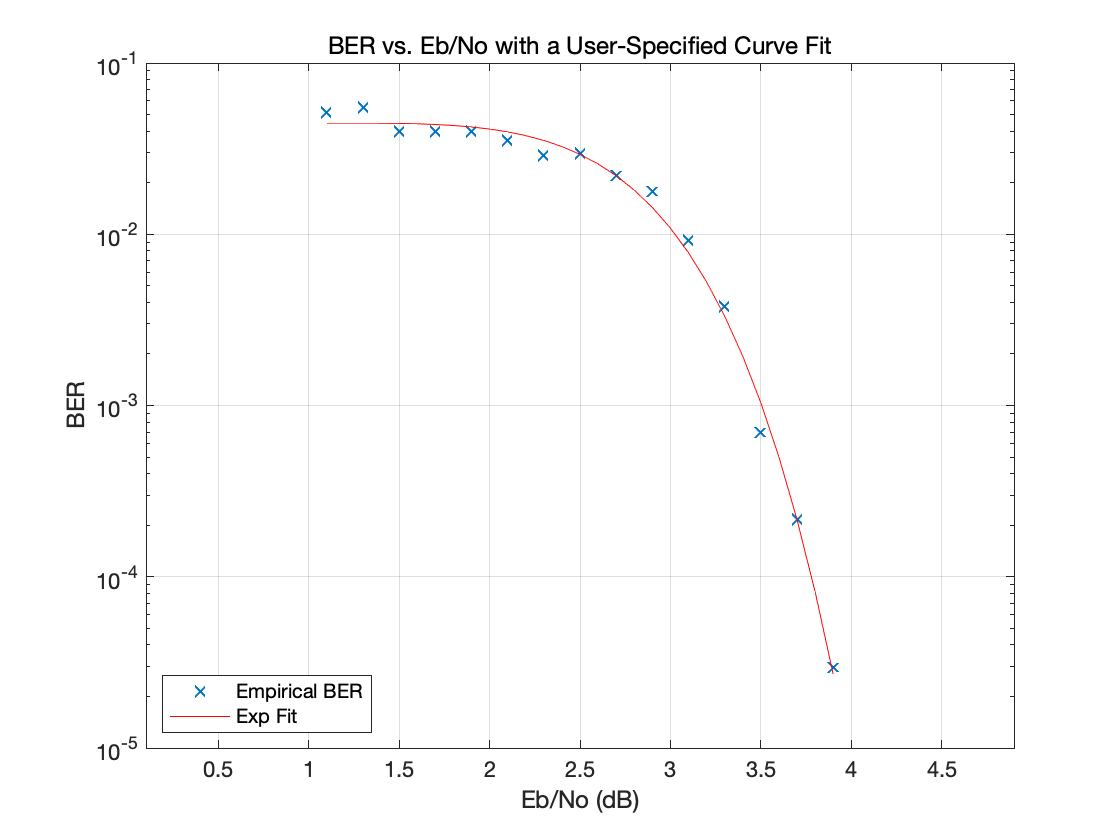
\includegraphics[width=3.1in]{figure/pg_bit_er.png}
    \caption{PG-LDPC Bit Error Rate vs. Eb/No}
    \label{fig:pg_bit_er}
    \end{minipage}%
    \begin{minipage}[t]{0.5\linewidth}
    \centering
    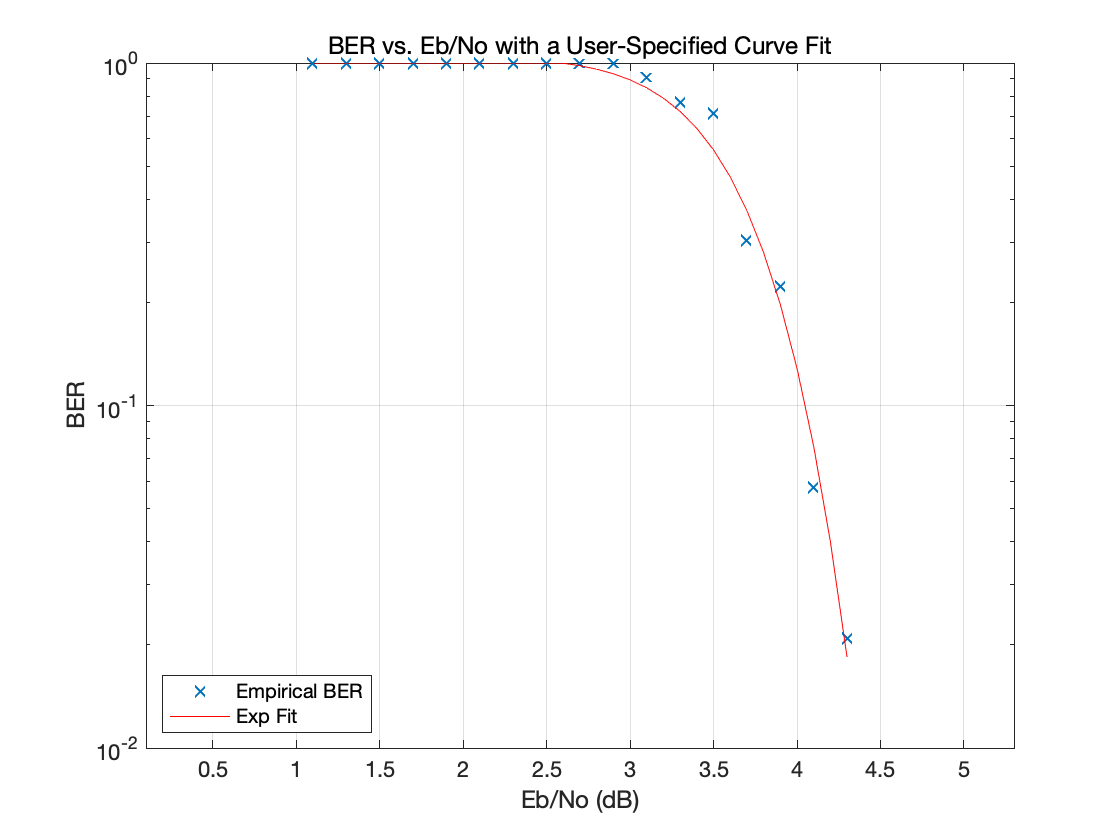
\includegraphics[width=3.1in]{figure/pg_block_er.png}
    \caption{PG-LDPC Block Error Rate vs. Eb/No}
    \label{fig:pg_block_er}
    \end{minipage}
    \end{figure}

\begin{figure}[htbp]
    \begin{minipage}[t]{0.5\linewidth}
    \centering
    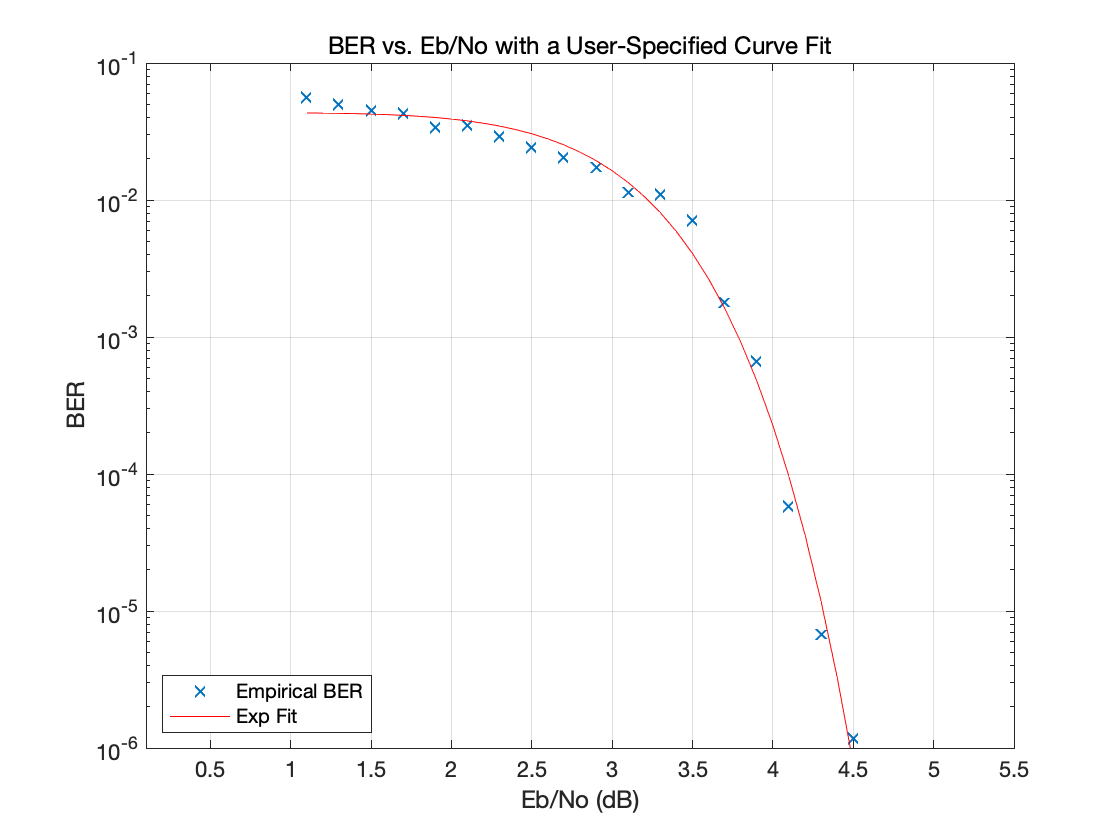
\includegraphics[width=3.1in]{figure/bj_bit_er.png}
    \caption{BJ-LDPC Bit Error Rate vs. Eb/No}
    \label{fig:bj_bit_er}
    \end{minipage}%
    \begin{minipage}[t]{0.5\linewidth}
    \centering
    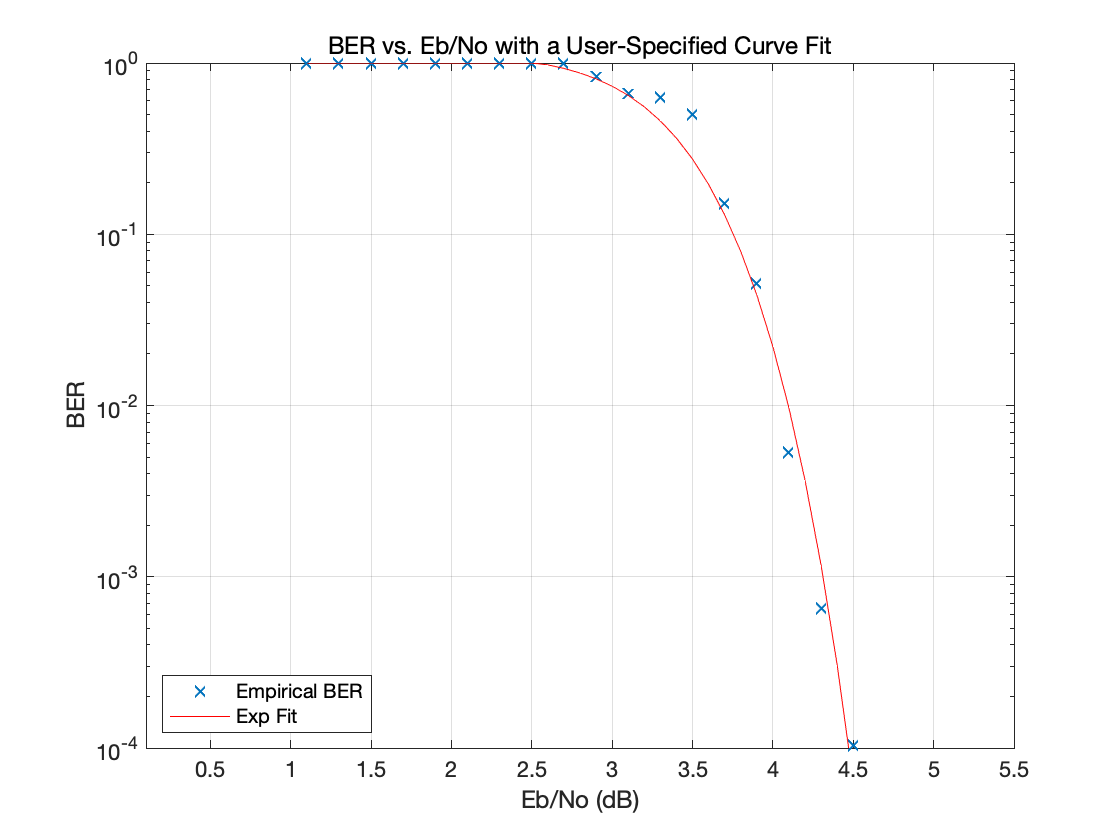
\includegraphics[width=3.1in]{figure/bj_block_er.png}
    \caption{BJ-LDPC Block Error Rate vs. Eb/No}
    \label{fig:bj_block_er}
    \end{minipage}
    \end{figure}

\begin{figure}[htbp]
    \begin{minipage}[t]{0.5\linewidth}
    \centering
    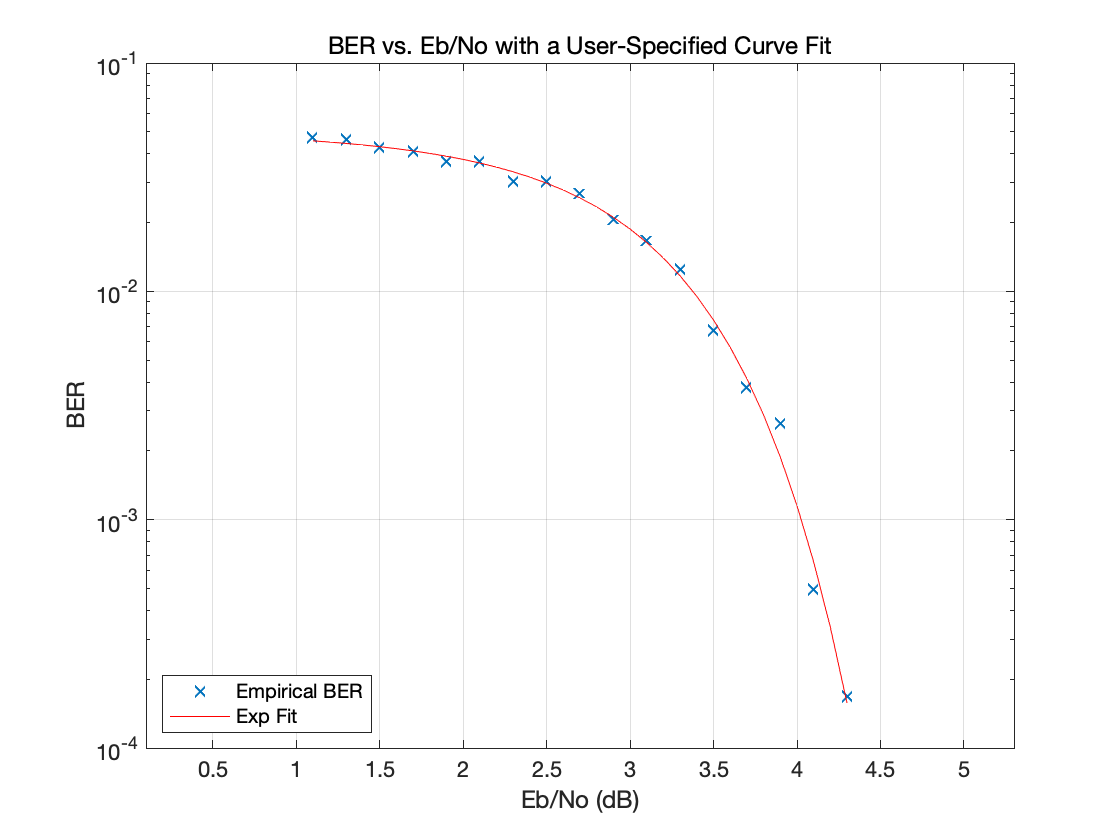
\includegraphics[width=3.1in]{figure/array_bit_er.png}
    \caption{Array-LDPC Bit Error Rate vs. Eb/No}
    \label{fig:array_bit_er}
    \end{minipage}%
    \begin{minipage}[t]{0.5\linewidth}
    \centering
    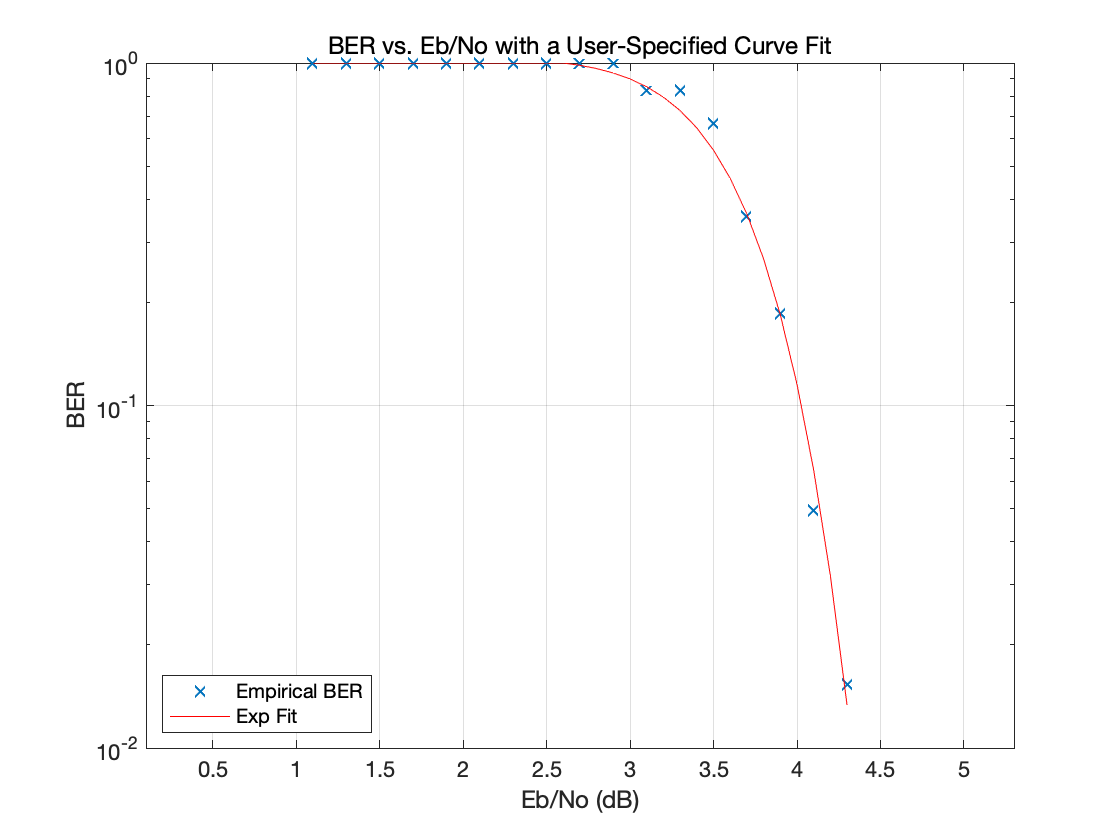
\includegraphics[width=3.1in]{figure/array_block_er.png}
    \caption{Array-LDPC Block Error Rate vs. Eb/No}
    \label{fig:array_block_er}
    \end{minipage}
    \end{figure}

    

\figref{fig:pg_bit_er}、\figref{fig:pg_block_er}为PG-LDPC 码的分组译码错误概率与比特译码错误概率曲线。
在信噪比小于3 dB时,比特错误译码概率较大,大致在(0.01, 0.1)区间;当信噪比超过3 dB时,比特译码错误概率呈指数级下降趋势。
当信噪比小于3 dB时,分组错误译码概率接近1;同样地,当信噪比超过3 dB时,分组译码错误概率呈指数级下降趋势。

\figref{fig:bj_bit_er}、\figref{fig:bj_block_er}为BJ-LDPC 码的分组译码错误概率
与比特译码错误概率曲线。\figref{fig:array_bit_er}、\figref{fig:array_block_er}
为ARRAY-LDPC 码的分组译码错误概率与比特译码错误概率曲线。BJ-LDPC与ARRAY-LDPC的比特译码
错误概率和分组译码错误概率的变换趋势与PG-LDPC的变化趋势基本一致。相比而言, 当信噪比逐渐
变大,PG-LDPC的分组译码效果更好,在信噪比为3.8 dB时,其错误概率可以低至 \(10^{-3}\),
而其余两种编码错误概率大于\(10^{-2}\)。在比特译码方面,也是 PG-LDPC 效果更好,在信噪比达到3.8 dB
时,它的错误概率低于\(10^{-5}\),其余两种编码的错误概率在\(10^{-3}\)左右。


\section{总结}
我们的实验主要分成四个部分。在前三部分,我们使用 matlab 分别构造投影平面循环LDPC码,基于
广义B-J码的准循环码和基于循环置换矩阵的Array LDPC码。第四部分我们实现迭代译码算法,可视化
并比较三种编码的分组译码错误概率和比特译码错误概率。通过比较,我们发现比特译码错误概率一致地低于
分组译码错误概率;PG-LDPC码在比特译码错误概率和分组译码错误概率上都表现更优越。










% \subsection{实验目的}

% 学习掌握神经网络相关原理,并将其应用于实际数据集的分类问题。
% \subsection{实验数据}

% MNIST数据集是由Yann Lecun提供的手写数字数据集,主要包含了60000张的训练图像和10000张的测试图像,囊括了各种手写数字图片。


% \begin{figure}[htbp]
%     \centering
%     \includegraphics[width=7cm]{figure/mnist_sample.png}
%     \caption{MNIST 图片示例 \label{fig:data}}
% \end{figure}



% \subsection{任务要求}

% \begin{enumerate}
%     \item 自己手动搭建神经网络,实现前后向,参数更新。神经网络结构不限,建议使用CNN;
%     \item 利用训练好的神经网络对测试集进行分类;
%     \item 依据初步的分类结果,对所设计的网络结构进行分析与改进;
%     \item 分析实验结果,与前两次实验(模式识别第一次实验和第二次实验)结果进行对比分析。
% \end{enumerate}

% \subsection{参考方案}

% \begin{enumerate}
%     \item 网络结构:卷积层 -> 激活层 ->池化层 ->全连接层->分类层;
%     \item 初始化:零均值正态分布;
%     \item 优化器:随机梯度下降 SGD;
%     \item 并行计算:将 conv 和 fc 转换为矩阵计算,代替循环计算。
% \end{enumerate}

% \subsection{注意事项}
% \begin{enumerate}
%     \item 独立完成;
%     \item 在实验报告中用图形方式展示所设计的网络结构;编程语言自选,代码中要包含神经网络搭建,训练及测试的基本步骤;
%     \item 上述为基本任务要求,占本次实验分数的百分之80。其余百分之20的分数,留给实验过程中独到的思考和创新点;
%     \item 实验报告提交为PDF格式。
% \end{enumerate}

% \section{实现方法}

% \subsection{总体说明}
% 使用 Python 与 numpy 实现了简单的神经网络,称为 numpy\_cnn。

% 神经网络的训练过程可以分为输入数据、前向传播、计算损失、反向传播梯度、更新参数几个阶段,而主要的运算则可以分为数据在网络层间的流动、损失的计算、参数的更新这三种。考虑到以上不同类型的运算,将numpy\_cnn分为了以下几个层次组件:
% \begin{itemize}
%     \item Tensor 张量:可学习参数使用Tensor,内部保存参数的值与梯度,底层直接使用 numpy 的 ndarray;数据与梯度也都用 numpy 的 ndarray 表示;
%     \item layers 网络层:网络层接收输入,进行运算并输出结果;所有的网络层都有前向传播与反向传播运算;
%     \item loss 损失函数:给定网络输出值与真实值,损失函数计算损失值与最后一层的梯度;
%     \item net 网络:网络将多个网络层组合起来,实现数据与梯度的流动;
%     \item optimizer 优化器:完成反向传播得到梯度后,使用优化器对可学习参数进行更新。
% \end{itemize}

% 基于实现的各个组件,整体的流程为:

% \begin{lstlisting}[frame=single, language=python, basicstyle=\footnotesize\menlo, caption=Pipeline\label{lst:pipeline}]
% # 构建网络、损失函数、优化器
% net = Net([layer1, layer2, ...])
% loss_f = CrossEntropyLoss()
% optimizer = Adam(net.parameters)

% # 训练过程
% for epoch in range(num_epochs):
%     for X, y in data_itetator():
%         # 前向传播
%         preds = net.forward(X)
%         # 计算 loss 与最后一层的梯度
%         l = loss_f.loss(preds, y)
%         grad = loss_f.grad(preds, y)
%         # 梯度反传
%         net.backward(grad)
%         # 参数更新
%         optimizer.update()

% # 推断过程
% test_preds = net.forward(X_test)
% \end{lstlisting}

% \subsection{各模块实现}

% \subsubsection{Tensor}

% 我们实现的Tensor很简单,就是把两个numpy.ndarray组合在了一起。如前面所说,可学习参数用Tensor,而net.parameters就是网络所有的可学习参数组成的列表,代码 \ref{lst:pipeline} 中我们将其传给了优化器。通过这种设计,优化器就可以用Tensor内的梯度对参数值进行更新,比较方便。

% \subsection{网络层}

% 我们主要实现了2维卷积、2维最大池化、全连接以及ReLU激活层。每个网络层都需要实现forward函数与backward函数,分别进行前向传播与反向传播的计算,代码 \ref{lst:pipeline} 中网络的前向传播与反向传播实际上就是依次调用各网络层的forward 与 backward 函数。

% 在实现的网络层中,全连接层与卷积层有可学习参数,而池化层与激活层则没有。全连接层中,我们在forward函数中计算$wx+b$,其中$x$、$w$、$b$分别为输入、权重和偏置,并将计算后的结果输出以便继续传递;而backward函数则接收来自后一层回传的梯度,并计算其关于$w$、$b$和$x$的梯度,关于$w$和$b$的梯度保存到相应Tensor中用于更新参数,而关于$x$的梯度则作为函数的返回值用于继续回传。

% 卷积层的实现中,除了上一段中提到的内容外,还要考虑 padding 的影响,也就是backward函数最后输出的应该是关于不进行padding的 $x$ 的梯度。此外,由于卷积操作中循环较多,直接计算效率很低,我们使用了著名的im2col方法,将卷积操作转化成了两个矩阵相乘,这两个矩阵分别对应与输入数据与卷积核。因为numpy对矩阵相乘等运算进行了很多优化,这种转化可以大大提升网络的效率。

% 池化层与激活层没有可学习参数,它们的backward函数只需计算后一层回传来的梯度对输入数据的梯度,再将计算得到的梯度输出即可。

% 在具体实现时,我们也参考了一些网上的博客与代码,如 \url{https://github.com/leeroee/NN-by-Numpy}。

% \subsection{损失函数}

% 损失函数需要计算损失值与关于预测值的梯度。因为要解决分类问题,我们实现了多分类问题中常用的Softmax交叉熵损失函数。

% 设模型的输出为$o$,类别数为$K$,可以使用Softmax计算概率分布,结果为
% \[\hat{y}_k = \frac{\exp(o_k)}{\sum_{k=1}^K \exp(o_k)}\]
% 而多分类下的交叉熵损失为
% \[J_{CE}(y,\hat{y}) = -\sum_{i=1}^N\sum_{k=1}^K y^{(i)}_k \log(\hat{y}^{(i)}_k)=-\sum_{i=1}^N \log(\hat{y}^{(i)}_c) = -\sum_{i=1}^N (o^{(i)}_c - \log(\sum_{k=1}^K\exp(o^{(i)}_k)))\]
% 其中$N$为样本数目,$c$表示真实类别。再求交叉熵损失$J_{CE}$关于$o$的梯度即可。

% \subsection{优化器}

% 代码 \ref{lst:pipeline} 中我们将网络的参数net.parameters传给了优化器。net.parameters是整个网络所有可学习参数Tensor的列表,在网络完成反向传播后,Tensor中保存着参数的值与梯度,利用 optimizer.update() 就对参数进行了更新。

% 开始时使用了随机梯度下降法SGD,但网络收敛比较慢。后来参考\cite{kingma2014adam}与\cite{zhang2019dive}实现了Adam算法,收敛速度快了很多。

% \subsection{网络参数初始化}

% 全连接层与卷积层的权重参数使用XavierUniform方法\cite{glorot2010understanding}进行初始化,而偏置参数则初始化为0。

% \section{实验与结果分析}

% 分别使用了一个只有全连接层与ReLU激活层的全连接网络和一个类似于LeNet的网络两种模型进行了实验。LeNet的网络结构如图所示。

% \begin{figure}[htbp]
% 	\centering
% 	\includegraphics[width=0.6\textwidth]{figure/lenet.png}
% 	\caption{LeNet 网络结构 \label{fig:lenet}}
% \end{figure}

% 我们的全连接网络使用了三个全连接层,两个激活层,称为fc-net,其网络定义为:
% \begin{lstlisting}[frame=single, language=python, basicstyle=\footnotesize\menlo]
% net = Net([
%     layers.Linear(784, 400),
%     layers.ReLU(),
%     layers.Linear(400, 100),
%     layers.ReLU(),
%     layers.Linear(100, 10)
% ])
% \end{lstlisting}

% 使用的卷积网络与LeNet比较像,但也有些差别,用了两个卷积层,三个全连接层,称为conv-net,其网络定义为:
% \begin{lstlisting}[frame=single, language=python, basicstyle=\footnotesize\menlo]
% net = Net([
%     layers.Conv2d(1, 6, k_size=(5, 5), stride=(1, 1), padding=(2, 2)),
%     layers.ReLU(),
%     layers.MaxPool2d(k_size=[2, 2], stride=[2, 2]),
%     layers.Conv2d(6, 16, k_size=[5, 5], stride=[1, 1]),
%     layers.ReLU(),
%     layers.MaxPool2d(k_size=[2, 2], stride=[2, 2]),
%     layers.Reshape(-1),
%     layers.Linear(400, 120),
%     layers.ReLU(),
%     layers.Linear(120, 84),
%     layers.ReLU(),
%     layers.Linear(84, 10)
% ])
% \end{lstlisting}

% 某次训练中,fc-net在14个epoch后,测试集准确率取得最佳结果,为 98.64\%;某次训练中,conv-net在12个epoch后取得最佳结果,为99.16\%。整体来看,conv-net的结果优于fc-net。不过,在我们的机器上,fc-net训练一个epoch只需要6.2秒左右,而conv-net一个epoch需要76秒左右。

% 在第一次实验中,使用PCA降为+贝叶斯判决+最大似然估计,最高的准确率为96.37;而第二次实验中,使用线性判别器进行二分类,一些易分类别准确率接近1,而有些类别则只有94\%左右。可见,神经网络方法确实优于传统方法。

% \section{总结}

% 本次实验,实现了一个简单的神经网络模型,学到了很多东西。感谢助教和老师一些学期的教导和帮助。

% \section{模板介绍}

% 此模板是基于 \LaTeX{} 的标准文类 article设计,也即意味着你可以把 article 文类的选项传递给本模板,比如 \lstinline{a4paper, 10pt} 等等(推荐使用 \lstinline{11pt})。本模板支持 \lstinline{PDFLaTeX} 和 \lstinline{XeLaTeX}\footnote{中文字体均使用 \lstinline{ctex} 包设置。} 两种编译方式。


% 数学字体的效果如下:
% \begin{equation}
% (a+3b)^{n} = \sum_{k=0}^{n} C_{n}^{k} a^{n-k} (3b)^k\label{eq:binom}
% \end{equation}
      
% \subsection{全局选项}
% 我在这个模板中定义了一个语言选项 \lstinline{lang},可以选择英文模式 \lstinline{lang=en}(默认)或者中文模式 \lstinline{lang=cn}。当选择中文模式时,图表的标题引导词以及参考文献,定理引导词等信息会变成中文。你可以通过下面两种方式来选择语言模式:
% \begin{lstlisting}
% \documentclass[lang=cn]{elegantpaper} % or
% \documentclass{cn}{elegantpaper} 
% \end{lstlisting}


% \subsection{自定义命令}
% 在此模板中,并没有修改任何默认的命令或者环境,所以,你可以在此模板使用原来的命令和环境。另外,我自定义了 4 个命令:
% \begin{enumerate}
% 	\item \lstinline{\email}:创建邮箱地址的链接;
% 	\item \lstinline{\figref}:用法和 \lstinline{\ref} 类似,但是会在插图的标题前添加 <\textbf{图 n}> ;
% 	\item \lstinline{\tabref}:用法和 \lstinline{\ref} 类似,但是会在表格的标题前添加 <\textbf{表 n}>;
% 	\item \lstinline{\keywords}:为摘要环境添加关键词。
% \end{enumerate}

% \subsection{列表环境}
% 你可以使用列表环境(\lstinline{itemize}、\lstinline{enumerate}、\lstinline{description}),示例如下:\\[2ex]
% \begin{minipage}[c]{0.59\linewidth}
% \begin{lstlisting}
% \begin{itemize}
%    \item Routing and resource discovery;
%    \item Resilient and scalable networks; 
%    \item Distributed storage and search.
% \end{itemize}
% \end{lstlisting}
% \end{minipage}
% \begin{minipage}[c]{0.4\linewidth}
% \begin{itemize}
%    \item Routing and resource discovery;
%    \item Resilient and scalable networks;
%    \item Distributed storage and search.
% \end{itemize}
% \end{minipage}


% \subsection{插图}
% 插图的命令和以前一样,也是使用 \lstinline{figure} 环境。\figref{fig:scatter} 显示了插图的效果。你可以把你的图放到当前工作目录的如下子目录下 (\lstinline{./image/}, \lstinline{./img/}, \lstinline{./figure/}, \lstinline{./fig/})。
% \begin{lstlisting}
% \begin{figure}[htbp]
% 	\centering
% 	\includegraphics[width=0.6\textwidth]{scatter.pdf}
% 	\caption{Scatter Plot Example \label{fig:scatter}}
% \end{figure}
% \end{lstlisting}
% \begin{figure}[htbp]
% 	\centering
% 	\includegraphics[width=0.6\textwidth]{scatter.pdf}
% 	\caption{Scatter Plot Example \label{fig:scatter}}
% \end{figure}




% \subsection{参考文献}
% 此模板使用了 Bib\TeX{} 来生成参考文献,默认使用的文献样式(bib style)是 \lstinline{GB/T 7714-2015}\footnote{通过调用 \href{https://ctan.org/pkg/gbt7714}{\lstinline{gbt7714}} 宏包}。参考文献示例:~\cite{en3} 使用了中国一个大型的 P2P 平台(人人贷)的数据来检验男性投资者和女性投资者在投资表现上是否有显著差异。

% 你可以在谷歌学术,Mendeley,Endnote 中获得文献条目(bib item),然后把它们添加到 \lstinline{wpref.bib} 中。在文中引用的时候,引用它们的键值(bib key)即可。注意需要在编译的过程中添加 Bib\TeX{} 编译。如果你想在参考文献中添加未引用的文献(部分或者全部),可以使用
% \begin{lstlisting}
% \nocite{EINAV2010, Havrylchyk2018} % add the two reference.
% \nocite{*}   % add all the reference in the bib file.
% \end{lstlisting}

% \section{示例}
% 在这部分,我提供一个示例文档:
% \begin{lstlisting}
% \documentclass[lang=cn]{elegantpaper}

% % title information
% \title{A Working Paper Example}
% \author{ddswhu} 
% \institute{Elegant\LaTeX{} Group}
% \version{1.00}
% \date{\today}

% \begin{document}

% \maketitle

% \begin{abstract}
% Your abstract goes here.
% \keywords{keyword1, keyword2}
% \end{abstract}

% \section{Introduction}
% The content of introduction section.

% \section{Conclusion}
% The content of conclusion section.

% % include the noncited reference
% \nocite{ref1, ref2}
% \bibliography{wpref}
% \end{document}
% \end{lstlisting}

% \nocite{*}
\bibliography{wpref}

\end{document}
